% Options for packages loaded elsewhere
\PassOptionsToPackage{unicode}{hyperref}
\PassOptionsToPackage{hyphens}{url}
%
\documentclass[
  12pt,
]{article}
\usepackage{lmodern}
\usepackage{amssymb,amsmath}
\usepackage{ifxetex,ifluatex}
\ifnum 0\ifxetex 1\fi\ifluatex 1\fi=0 % if pdftex
  \usepackage[T1]{fontenc}
  \usepackage[utf8]{inputenc}
  \usepackage{textcomp} % provide euro and other symbols
\else % if luatex or xetex
  \usepackage{unicode-math}
  \defaultfontfeatures{Scale=MatchLowercase}
  \defaultfontfeatures[\rmfamily]{Ligatures=TeX,Scale=1}
\fi
% Use upquote if available, for straight quotes in verbatim environments
\IfFileExists{upquote.sty}{\usepackage{upquote}}{}
\IfFileExists{microtype.sty}{% use microtype if available
  \usepackage[]{microtype}
  \UseMicrotypeSet[protrusion]{basicmath} % disable protrusion for tt fonts
}{}
\makeatletter
\@ifundefined{KOMAClassName}{% if non-KOMA class
  \IfFileExists{parskip.sty}{%
    \usepackage{parskip}
  }{% else
    \setlength{\parindent}{0pt}
    \setlength{\parskip}{6pt plus 2pt minus 1pt}}
}{% if KOMA class
  \KOMAoptions{parskip=half}}
\makeatother
\usepackage{xcolor}
\IfFileExists{xurl.sty}{\usepackage{xurl}}{} % add URL line breaks if available
\IfFileExists{bookmark.sty}{\usepackage{bookmark}}{\usepackage{hyperref}}
\hypersetup{
  pdftitle={Turnout and Amendment 4},
  pdfauthor={Kevin Morris},
  hidelinks,
  pdfcreator={LaTeX via pandoc}}
\urlstyle{same} % disable monospaced font for URLs
\usepackage[margin=1in]{geometry}
\usepackage{longtable,booktabs}
% Correct order of tables after \paragraph or \subparagraph
\usepackage{etoolbox}
\makeatletter
\patchcmd\longtable{\par}{\if@noskipsec\mbox{}\fi\par}{}{}
\makeatother
% Allow footnotes in longtable head/foot
\IfFileExists{footnotehyper.sty}{\usepackage{footnotehyper}}{\usepackage{footnote}}
\makesavenoteenv{longtable}
\usepackage{graphicx}
\makeatletter
\def\maxwidth{\ifdim\Gin@nat@width>\linewidth\linewidth\else\Gin@nat@width\fi}
\def\maxheight{\ifdim\Gin@nat@height>\textheight\textheight\else\Gin@nat@height\fi}
\makeatother
% Scale images if necessary, so that they will not overflow the page
% margins by default, and it is still possible to overwrite the defaults
% using explicit options in \includegraphics[width, height, ...]{}
\setkeys{Gin}{width=\maxwidth,height=\maxheight,keepaspectratio}
% Set default figure placement to htbp
\makeatletter
\def\fps@figure{htbp}
\makeatother
\setlength{\emergencystretch}{3em} % prevent overfull lines
\providecommand{\tightlist}{%
  \setlength{\itemsep}{0pt}\setlength{\parskip}{0pt}}
\setcounter{secnumdepth}{5}
\usepackage{rotating}
\usepackage{setspace}\doublespacing
\newcommand{\beginsupplement}{\setcounter{table}{0}  \renewcommand{\thetable}{A\arabic{table}} \setcounter{figure}{0} \renewcommand{\thefigure}{A\arabic{figure}}}
\usepackage{booktabs}
\usepackage{longtable}
\usepackage{array}
\usepackage{multirow}
\usepackage{wrapfig}
\usepackage{float}
\usepackage{colortbl}
\usepackage{pdflscape}
\usepackage{tabu}
\usepackage{threeparttable}
\usepackage{threeparttablex}
\usepackage[normalem]{ulem}
\usepackage{makecell}
\usepackage{xcolor}
\newlength{\cslhangindent}
\setlength{\cslhangindent}{1.5em}
\newenvironment{cslreferences}%
  {\setlength{\parindent}{0pt}%
  \everypar{\setlength{\hangindent}{\cslhangindent}}\ignorespaces}%
  {\par}

\title{Turnout and Amendment 4\thanks{The author thanks Many People for their comments on this project. All errors are my responsibility.}}
\author{Kevin Morris\footnote{Researcher, Brennan Center for Justice at NYU School of Law, 120 Broadway Ste 1750, New York, NY 10271 (\href{mailto:kevin.morris@nyu.edu}{\nolinkurl{kevin.morris@nyu.edu}})}}
\date{February 10, 2020}

\begin{document}
\maketitle
\begin{abstract}
Here is an abstract.
\end{abstract}

\pagenumbering{gobble}
\pagebreak

\pagenumbering{arabic}

\hypertarget{introduction}{%
\section*{Introduction}\label{introduction}}
\addcontentsline{toc}{section}{Introduction}

On November 6\textsuperscript{th}, 2018, Floridians voted to amend their state constitution to allow individuals with felony convictions in their past (Taylor \protect\hyperlink{ref-Taylor2018}{2018}). The move was hailed as transformational for Floridian --- and American --- democracy (Morris \protect\hyperlink{ref-Morris2018}{2018}); the Sentencing Project (\protect\hyperlink{ref-sentencing_2016}{2016}) had estimated a few years earlier that some 1.5 million Floridians were disenfranchised and had finished serving their sentences. The racial implications for the constitutional amendment were also clear: according to the same Sentencing Project report, more than 1 out of every 5 Black Floridians was prohibited from democratic participation thanks to the state's disenfranchisement policies. The Amendment received broad support. Although it needed just 60 percent of the vote to pass, precinct-level data from the Florida Division of Elections shows that 64.5 percent of voters supported the ballot initiative. Conversely, the winning candidates for Governor and United States Senate won just 49.5 and 49.9 percent of the vote, respectively, implying that the constitutional amendment enjoyed some bipartisan support.

Felony disenfranchisement is not unique to Florida's electoral system: in all but two states in the United States, individuals convicted of felony offenses lose their right to vote for at least some period of time (Brennan Center for Justice \protect\hyperlink{ref-bcj_laws}{2019}). According to the Brennan Center for Justice, felony convictions result in lifetime prohibitions from voting for some citizens in 11 states based on the severity of the crime.\footnote{Iowa stands alone in disenfranchising all individuals ever convicted of felony offenses.} Nevertheless, the shift in Florida from permanent disenfranchisement for all individuals convicted of felony offenses to restoring voting rights to most individuals\footnote{Individuals convicted of felony sexual assault or murder remain permanently disenfranchised} upon the termination of their sentence moved the needle significantly: according to the same Sentencing Project report, post-sentence Floridians accounted for roughly 24 percent of all disenfranchised Americans (Uggen, Larson, and Shannon \protect\hyperlink{ref-sentencing_2016}{2016}).

The case of Amendment 4 was somewhat unique in how Floridians with felony convictions in their past had their voting rights restored. Usually, the question of voting rights restoration is not put directly to the voters. In New York State in 2018 and Kentucky in 2019, for instance, governors signed executive order restoring voting rights to some disenfranchised individuals (Wang \protect\hyperlink{ref-Wang2018}{2018}; Wines \protect\hyperlink{ref-Wines2019}{2019}). In other states such as Louisiana (Crisp \protect\hyperlink{ref-Crisp2019}{2019}) and Colorado (Baumann \protect\hyperlink{ref-Baumann2019}{2019}), state lawmakers have passed bills restoring voting rights to formerly incarcerated individuals. In Florida, however, put the question was put directly to voters. In the Sunshine State, voters had the opportunity to democratically decide whether they wanted to restore voting rights to their formerly incarcerated or probationed neighbors.

This paper explores whether the presence of Amendment 4 on the ballot increased participation among individuals who live in close proximity to the disenfranchised. There is much literature that establishes that proximal contact with the criminal justice system reduces eligible Americans' propensity to vote (e.g.~Ochs \protect\hyperlink{ref-Ochs2006}{2006}; Bowers and Preuhs \protect\hyperlink{ref-Bowers2009}{2009}; Burch \protect\hyperlink{ref-Burch2013}{2013}; King and Erickson \protect\hyperlink{ref-King2016}{2016}). Little work, however, has been done exploring whether the re-enfranchisement of family and community members can bring back these lost votes. The case of Amendment 4 in Florida offers a unique opportunity to investigate whether these eligible individuals can be reincorporated into our democratic processes.

\hypertarget{theory-and-literature}{%
\section*{Theory and Literature}\label{theory-and-literature}}
\addcontentsline{toc}{section}{Theory and Literature}

\hypertarget{democratic-withdrawal}{%
\subsection*{Democratic Withdrawal}\label{democratic-withdrawal}}
\addcontentsline{toc}{subsection}{Democratic Withdrawal}

\hypertarget{self-interested-voting}{%
\subsection*{Self-Interested Voting}\label{self-interested-voting}}
\addcontentsline{toc}{subsection}{Self-Interested Voting}

\hypertarget{research-design}{%
\section*{Research Design}\label{research-design}}
\addcontentsline{toc}{section}{Research Design}

I begin by testing whether neighborhoods the number of formerly incarcerated individuals living in a neighborhood influenced the turnout in 2018 of that neighborhood. ``Neighborhoods'' and ``turnout'' are defined in multiple ways throughout the neighborhood analysis --- each definition suffers slightly because of data limitations, but together they paint a full picture.

I begin by defining neighborhoods as precincts. Defining neighborhoods as precincts provides two benefits: firstly, because the Florida Division of Elections produces results at this level, we can identify not only how many people cast a ballot at all, but also how many people participated in the contest for Amendment 4. This is an important distinction: voters are more likely to vote for the top-line contests for Governor and United States Senator, and ``roll-off'' (that is, abstain from participating) when it comes to downballot questions such as ballot initiatives {[}CITE{]}. Given that some research indicates that Black voters are more likely to roll-off than white voters (Vanderleeuw and Engstrom \protect\hyperlink{ref-Vanderleeuw1987}{1987}, but see @Knack2008), the question of roll-off is of particular interest when considering a question that intersects with race such as the criminal justice system. Precinct-level data, therefore, allows us to determine not how many voters in a neighborhood voted for \emph{any} contest, but specifically for Amendment 4.

Precinct-level data also allows us to tell the extent to which neighborhoods supported Amendment 4. The secret ballot, of course, prevents us from knowing how individuals voted; precinct-level data, therefore, offer the lowest-level picture of what sorts of communities were more or less likely to support Amendment 4.

Unfortunately, the use of precinct-level data leaves us with a major drawback: when doing analysis at this level, bias-free turnout denominators are hard to come by. Because the Census Bureau does not produce population estimates for individual voting precincts, turnout cannot be calculated by dividing the number of ballots cast by the eligible population; turnout, rather, has to be constructed as a share of registered voters. If there is a relationship between the independent variable of interest and the registration rate of a neighborhood, this could bias our estimates. In other words, if turnout among \emph{registered voters} is the same in two neighborhoods, but one neighborhood has a higher registration rate, that neighborhood has a higher true turnout rate --- but that fact cannot be uncovered using precinct-level data.

To sidestep this potential problem, I also define neighborhoods as Census block groups. The Census makes estimates of the citizen voting-age population available at this level, providing a better denominator for calculating turnout. In this case, however, I must use a geocoded voter file to determine turnout. Thus, because I aggregate the number of ballots cast in a block group from individual level data, I am unable to determine whether an individual actually participated in the contest for Amendment 4 or they rolled off. Similarly, I am unable to interrogate the relationship between block group characteristics and support for Amendment 4.

After examining whether the presence of formerly incarcerated individuals was related with a \emph{neighborhood's} turnout rate, I ask whether the individuals with the potentially closest relationship to the disenfranchised voters were more likely to turnout. For this analysis, I use release addresses provided to the DOC and voter file data to identify registered voters who live with formerly incarcerated individuals. Voters are considered ``treated'' if they live with a formerly incarcerated individual, and ``untreated'' otherwise. I then use a variety of individual- and neighborhood-level characteristics to match treated and untreated voters using a genetic algorithm (Sekhon \protect\hyperlink{ref-Sekhon2011}{2011}). After matching these voters, I employ a difference-in-differences specification to determine whether treated voters participated at higher rates in the 2018 election.

\hypertarget{data}{%
\section*{Data}\label{data}}
\addcontentsline{toc}{section}{Data}

I leverage multiple data sources to investigate whether individuals in proximate contact with disenfranchised residents were more likely to vote in the 2018 election.

\hypertarget{department-of-corrections-data}{%
\subsection*{Department of Corrections Data}\label{department-of-corrections-data}}
\addcontentsline{toc}{subsection}{Department of Corrections Data}

Data from the Florida Department of Corrections is used to identify individuals who have been to prison in Florida. These records include all individuals released from prison since October 1, 1997.\footnote{Using the last-known address for individuals last released from prison in 1997 presents some difficulty; it is possible that the formerly incarcerated individuals have died or moved. In Appendix A, I show that the results presented in the body of this article continue to hold even when limiting the pool of formerly incarcerated people to individuals released from prison during or after 2015.} Using records of individuals currently in prison or on parole, I can identify all individuals who had been to prison but were not serving a sentence at the time of the 2018 midterm election. These are the individuals who would be re-enfranchsied by Amendment 4, and therefore the people most likely to encourage their friends and neighbors to vote on their behalf. I include only individuals with a valid release; individuals who died or absconded before their sentence was completed are removed from the dataset. I identify 342,694 such individuals.

The Florida Department of Corrections provides the last-known addresses of all individuals who were formerly incarcerated. The address data, however, are messy. In some cases, the address field is left blank; in others, the records simply notes the road or the town of the former inmate, without providing full address information. These addresses require substantial cleaning.

I begin the cleaning process by removing all records where the address does not begin with an integer. In other words, I assume that any record that begins with a letter does not have a fill address and cannot be used. I then geocode these addresses using Google Maps' geocoder, and drop all individuals whose addresses could not be geocoded or were geocoded outside of Florida. The resulting list includes 286,268. This represents 83.5 percent of the formerly incarcerated individuals. The failure to identify the home location of so many formerly incarcerated individuals may pose problems; if we end up undercounting the number of formerly incarcerated individuals in some neighborhoods, we may underestimate the effects of the presence of formerly incarcerated individuals on neighborhood or individual level turnout.

Many formerly incarcerated individuals leave prison not for homes with family members, but rather to homeless shelters and halfway houses. The body of this paper excludes formerly incarcerated individuals whose last known address was also listed by five or more other individuals, because neighborhoods may respond differently to institutions for returning citizens than the return of a family or community member. Appendix B demonstrates that the primary findings in the paper hold when we include all formerly incarcerated individuals, even if they returned to the same location as many other formerly incarcerated individuals.

The successfully geocoded, formerly incarcerated individuals are then mapped to their home Census block groups using shapefiles from the Census Bureau, and to their home voter precincts using data collected by Kelso and Migurski (\protect\hyperlink{ref-Kelso2018}{2018}).

Statewide data on individuals who formerly served a term on felony probation are not available. This too may pose a problem for this study; neighborhoods with disenfranchised former probationers are also ``treated.'' Such data is available, however from COUNTY COUNTY. In Appendix C, I incorporate these data to interrogate whether the omission of these individuals from the statewide analyses is likely impacting my results.

\hypertarget{voter-file-data}{%
\subsection*{Voter File Data}\label{voter-file-data}}
\addcontentsline{toc}{subsection}{Voter File Data}

Individual-level voter file data are used for a variety of purposes in this analysis. I primarily use Florida voter file data from the data vendor L2. This file includes information on individuals such as their home address, their age and gender, their participation history, and their political affiliation. L2 also geocodes voters to their home Census blocks, and provides latitude and longitudes.

Although the L2 data includes estimates of voters' race and ethnicity, the raw Florida voter file includes self-identificated race and ethnicity. In place of L2's estimates, I use the self-reported data found in the raw Florida voter file (the two lists can be joined using a unique identifier). I also use the raw Florida file to provide the gender for voters for whom L2 did not have an estimate, as well as voters' home counties and precincts.

Precinct and block group demographics are constructed using the voter file data. A precinct's average age, therefore, is the average age of all voters registered in that precinct; the same is true for Census block groups. Some information such as median income, however, is not available at the individual level. For these variables, voters are assigned the median income (or education level, et cetera) of their home block group; the precinct average income, therefore, is effectively the average of all the block groups within that precinct, weighted by the number of registered voters in each block group.

For the individual-level analyses, I use individual-level demographic controls obtained from the voter files, and neighborhood-level demographic controls like income from the voter's block group.

\hypertarget{division-of-election-results-data}{%
\subsection*{Division of Election Results Data}\label{division-of-election-results-data}}
\addcontentsline{toc}{subsection}{Division of Election Results Data}

As discussed above, the Florida Division of Elections makes precinct-level results data available. These data come with precinct identifiers that correspond to the precinct reported in the Florida voter file.

\hypertarget{matched-department-of-corrections-and-voter-file-data}{%
\subsection*{Matched Department of Corrections and Voter File Data}\label{matched-department-of-corrections-and-voter-file-data}}
\addcontentsline{toc}{subsection}{Matched Department of Corrections and Voter File Data}

Identifying eligible registered voters who lived with formerly incarcerated individuals in the 2018 election requires matching on addresses. As discussed above, these addresses are often in different formats. To increase the quality of the matches, I standardize common street and address abbreviations as well as capitalization. ``Boulevard,'' for instance, becomes ``BLVD'' in each instance in the DOC and voter file data. These standardizations are taken from Appendix C of the USPS Postal Addressing Standards (\protect\hyperlink{ref-USPS2015}{2015}). Exact matching is required.

\hypertarget{results}{%
\section*{Results}\label{results}}
\addcontentsline{toc}{section}{Results}

I begin by examining whether --- and to what extant --- neighborhoods with formerly incarcerated individuals differ from neighborhoods elsewhere in the state. A simple comparison of neighborhoods with and without formerly incarcerated individuals, however, proves unhelpful: 97.4 percent of block groups in the state are home to someone who has been to prison, lending credence to the notion that the criminal justice system impacts nearly every neighborhood in the Sunshine State. There are, however, neighborhoods where formerly incarcerated individuals are concentrated. In Table \ref{tab:demos}, I weight the characteristics of each block group in the state by the number of formerly incarcerated individuals who live there. These are compared to the characteristics of all block groups in the state, weighted by total population.

\input{"../temp/table_whatever2.tex"}

Although nearly all parts of the state are impacted by the criminal justice system (and, more specifically, mass incarceration), Table \ref{tab:demos} makes clear that individuals return home to neighborhoods with lower incomes, higher levels of unemployment, and where a much larger share of the population is Black than other neighborhoods.

I now test whether the presence of formerly incarerated individuals impacted whether and how neighborhoods voted. I start by exploring the relationship between the number of formerly incarcerated individuals living in a neighborhood and neighborhood support for Amendment 4. Unsurprisingly, as Table \ref{tab:support-reg} makes clear, neighborhoods with higher numbers of disenfranchised individuals supported Amendment 4 at higher rates. Table \ref{tab:support-reg} presents OLS estimates with robust standard errors clustered at the United States congressional district level.\footnote{Where a precinct crosses district lines, it is assigned to the district that is home to the largest number of registered voters in the precinct.}

\begin{singlespace}

\input{"../temp/table1.tex"}
\end{singlespace}

Okay now the marginal effects plot

\begin{figure}[H]

{\centering 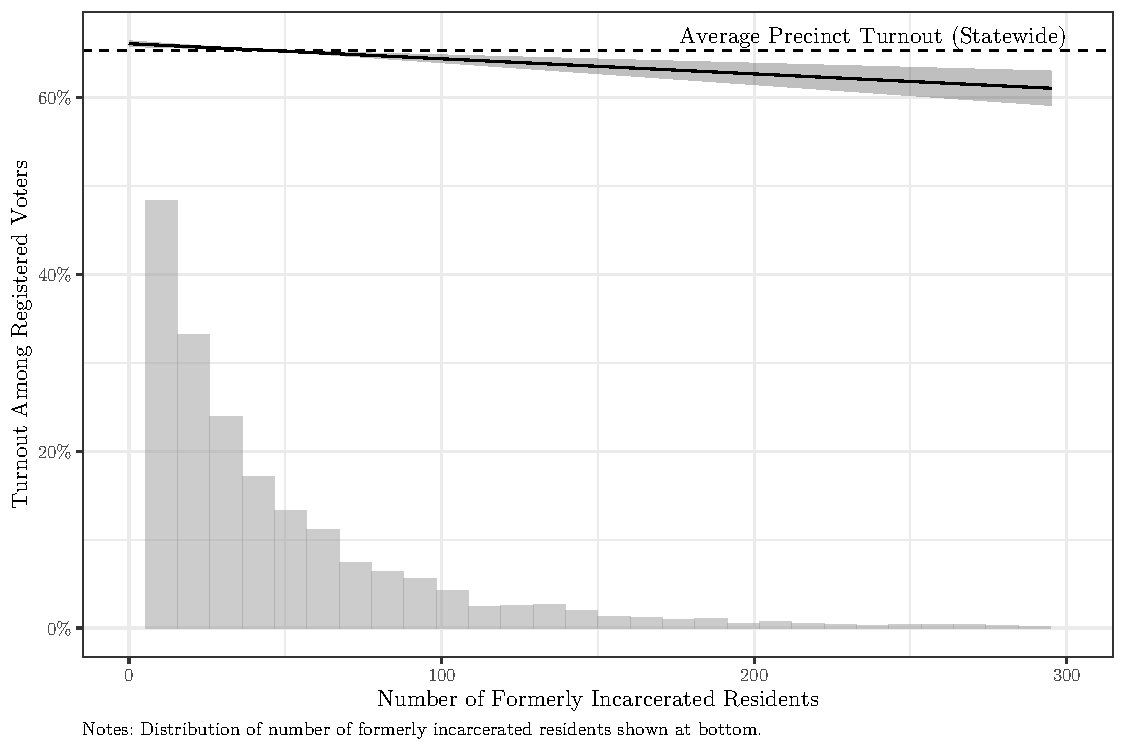
\includegraphics{write_files/figure-latex/marg1-1} 

}

\caption{\label{fig:marg1}Marginal Effect of Formerly Incarcerated Residents on Precinct Support for Amendment 4}\label{fig:marg1}
\end{figure}

\newpage

\hypertarget{references}{%
\section*{References}\label{references}}
\addcontentsline{toc}{section}{References}

\hypertarget{refs}{}
\begin{cslreferences}
\leavevmode\hypertarget{ref-Baumann2019}{}%
Baumann, Joella. 2019. ``Paroled Coloradans Are Now Eligible to Vote.'' \emph{Colorado Public Radio}, July.

\leavevmode\hypertarget{ref-Bowers2009}{}%
Bowers, Melanie, and Robert R. Preuhs. 2009. ``Collateral Consequences of a Collateral Penalty: The Negative Effect of Felon Disenfranchisement Laws on the Political Participation of Nonfelons*.'' \emph{Social Science Quarterly} 90 (3): 722--43. \url{https://doi.org/10.1111/j.1540-6237.2009.00640.x}.

\leavevmode\hypertarget{ref-bcj_laws}{}%
Brennan Center for Justice. 2019. ``Criminal Disenfranchisement Laws Across the United States.'' https://www.brennancenter.org/our-work/research-reports/criminal-disenfranchisement-laws-across-united-states.

\leavevmode\hypertarget{ref-Burch2013}{}%
Burch, Traci R. 2013. ``Effects of Imprisonment and Community Supervision on Neighborhood Political Participation in North Carolina:'' \emph{The ANNALS of the American Academy of Political and Social Science}, November. \url{https://doi.org/10.1177/0002716213503093}.

\leavevmode\hypertarget{ref-Crisp2019}{}%
Crisp, Elizabeth. 2019. ``Thousands of Felons in Louisiana Will Regain Voting Rights When This Law Takes Effect March 1.'' \emph{The Advocate}, February.

\leavevmode\hypertarget{ref-Kelso2018}{}%
Kelso, Nathaniel, and Michael Migurski. 2018. ``Election-Geodata.'' \emph{Election-Geodata}. https://github.com/nvkelso/election-geodata.

\leavevmode\hypertarget{ref-King2016}{}%
King, Bridgett A., and Laura Erickson. 2016. ``Disenfranchising the Enfranchised: Exploring the Relationship Between Felony Disenfranchisement and African American Voter Turnout.'' \emph{Journal of Black Studies}, July. \url{https://doi.org/10.1177/0021934716659195}.

\leavevmode\hypertarget{ref-Knack2008}{}%
Knack, Stephen, and Martha Kropf. 2008. ``Roll-Off at the Top of the Ballot: International Undervoting in American Presidential Elections.'' \emph{Politics \& Policy} 31 (4): 575--94. \url{https://doi.org/10.1111/j.1747-1346.2003.tb00163.x}.

\leavevmode\hypertarget{ref-Morris2018}{}%
Morris, Kevin. 2018. ``A Transformative Step for Democracy in Florida.'' \emph{Brennan Center for Justice}.

\leavevmode\hypertarget{ref-Ochs2006}{}%
Ochs, Holona Leanne. 2006. ``\,`Colorblind' Policy in Black and White: Racial Consequences of Disenfranchisement Policy.'' \emph{Policy Studies Journal} 34 (1): 81--93. \url{https://doi.org/10.1111/j.1541-0072.2006.00146.x}.

\leavevmode\hypertarget{ref-Sekhon2011}{}%
Sekhon, Jasjeet S. 2011. ``Multivariate and Propensity Score Matching Software with Automated Balance Optimization: The Matching Package for R.'' \emph{Journal of Statistical Software} 42 (1): 1--52. \url{https://doi.org/10.18637/jss.v042.i07}.

\leavevmode\hypertarget{ref-Taylor2018}{}%
Taylor, Adam. 2018. ``Florida's Move to Allow Ex-Felons to Vote Brings U.S. Closer to International Election Norms.'' \emph{Washington Post}, November.

\leavevmode\hypertarget{ref-sentencing_2016}{}%
Uggen, Christopher, Ryan Larson, and Sarah Shannon. 2016. ``6 Million Lost Voters: State-Level Estimates of Felony Disenfranchisement, 2016.'' Research Report. The Sentencing Project.

\leavevmode\hypertarget{ref-USPS2015}{}%
USPS. 2015. ``Appendix C.'' \emph{Postal Addressing Standards}. https://pe.usps.com/text/pub28/28apc\_002.htm.

\leavevmode\hypertarget{ref-Vanderleeuw1987}{}%
Vanderleeuw, James M., and Richard L. Engstrom. 1987. ``Race, Referendums, and Roll-Off.'' \emph{The Journal of Politics} 49 (4): 1081--92. \url{https://doi.org/10.2307/2130785}.

\leavevmode\hypertarget{ref-Wang2018}{}%
Wang, Vivian. 2018. ``Cuomo Plans to Restore Voting Rights to Paroled Felons.'' \emph{The New York Times}, April.

\leavevmode\hypertarget{ref-Wines2019}{}%
Wines, Michael. 2019. ``Kentucky Gives Voting Rights to Some 140,000 Former Felons.'' \emph{The New York Times}, December.
\end{cslreferences}

\end{document}
